\documentclass{article}

\usepackage{fullpage}
\usepackage[utf8]{inputenc}
\usepackage[american]{babel}
\usepackage{csquotes}
\usepackage{listings}
\usepackage[table]{xcolor}
\usepackage{amssymb}
\usepackage{amsmath}
\usepackage{fancyhdr}
\usepackage{lastpage}
\usepackage{parskip}
\usepackage{abstract}
\usepackage{url}
\usepackage{float}
\usepackage{enumitem}
\usepackage{fancybox}
\usepackage{amsmath}
\usepackage{graphicx}
\usepackage[bottom]{footmisc}
\usepackage{hyperref}
\usepackage{makecell}

\usepackage[backend=bibtex]{biblatex}
\bibliography{report}


% constants
\newcommand{\COURSE}{Bachelor Thesis}
\newcommand{\TITLE}{Abstract Machine}
\newcommand{\DATE}{June 2015}


%%% Local Variables:
%%% mode: latex
%%% TeX-master: "report"
%%% End:

% generalized stuff
\newcommand{\code}[1]{\texttt{#1}}
\newcommand{\term}[1]{\textit{#1}}

% colors
\definecolor{Brown}{cmyk}{0,0.81,1,0.60}
\definecolor{OliveGreen}{cmyk}{0.64,0,0.95,0.40}
\definecolor{CadetBlue}{cmyk}{0.62,0.57,0.23,0}
\definecolor{lightlightgray}{gray}{0.95}
\definecolor{lightgray}{gray}{0.85}
\definecolor{sh_comment}{rgb}{0.12, 0.38, 0.18}
\definecolor{sh_keyword}{rgb}{0.37, 0.38, 0.75}
\definecolor{sh_string}{rgb}{0.06, 0.10, 0.98}

% listings
\lstset{
  basicstyle=\small\ttfamily,
  stringstyle=\color{sh_string},
  keywordstyle = \color{sh_keyword}\bfseries,
  commentstyle=\color{sh_comment},
  backgroundcolor=\color{lightlightgray},
  frame=single,
  rulecolor=\color{lightgray},
  framesep=3pt,
  numbersep=5pt,
  xleftmargin=10pt,
  xrightmargin=10pt,
  showspaces=false,
  showstringspaces=false,
  tabsize=4,
  aboveskip=5pt,
  belowskip=5pt,
  lineskip=2pt,
  captionpos=b,
  numbers=left,
  numberstyle=\tiny,
  stepnumber=1,
  numbersep=100pt,
  breaklines,
  numbersep=5pt,
  breakatwhitespace=false,
  showspaces=false,
  showtabs=false
}

 % TODO
\lstdefinelanguage{bytecode}{
  keywords={fn, pop},
  keywordstyle=\color{blue}\bfseries,
  ndkeywords={class, export, boolean, throw, implements, import, this},
  ndkeywordstyle=\color{darkgray}\bfseries,
  identifierstyle=\color{black},
  sensitive=false,
  comment=[l]{//},
  morecomment=[s]{/*}{*/},
  commentstyle=\color{purple}\ttfamily,
  stringstyle=\color{red}\ttfamily,
  morestring=[b]',
  morestring=[b]"
}

\let\oldcite=\cite
\renewcommand\cite[1]{\ifthenelse{\equal{#1}{NEEDED}}{[citation~needed]}{\oldcite{#1}}}



\pagestyle{fancy}
\fancyhf{}
\setlength{\parindent}{0pt}
\setlength{\headheight}{15pt}
\setlength{\headsep}{25pt}
\lhead{\COURSE}
\chead{\TITLE}
\rhead{\DATE}
\cfoot{Page \thepage{} of~\pageref{LastPage}}


\begin{document}
%%% Local Variables:
%%% mode: latex
%%% TeX-master: "report"
%%% End:

\newcommand*\formatname[2]{
  \leavevmode
  \rlap{\textit{#1}}
  \hspace{0.3\linewidth}
  \code{#2}}

\begin{titlepage}

\thispagestyle{empty}

\begin{flushright}
  
\includegraphics[width=9cm]{images/dtu}
\end{flushright}

\vskip20mm
\begin{center}
  \vskip5mm
  \huge\textbf{\TITLE}
  \vskip5mm
  \Large \COURSE
  \vskip3mm
  \large \DATE
\end{center}
\vfill

\begin{flushleft}
  \normalsize
  \formatname{Markus Veie Færevaag}{s123692} \par
  \formatname{Simon Altschuler}{s123563} \par
  \vskip2cm
  
\includegraphics[width=7cm]{images/dtu-compute}
\end{flushleft}

\end{titlepage}

\clearpage

\tableofcontents
\clearpage

\section{Introduction}
\label{sec:intro}
%%% Local Variables:
%%% mode: latex
%%% TeX-master: "../report"
%%% End:

% Motivation

New programming languages are coming into existence at a very rapid pace. Tools
for creating languages are in abundance, and even the beginning student of
computer science will most likely posses the knowledge to use them. When
languages become pass\'e or fundamental shortcomings are discovered, the
prevalent solution seems to be the creation of new and improved languages
instead of updating the existing. All of this has resulted in hundreds, if not
thousands, of available languages in a myriad of styles and paradigms for just
as many different purposes.

The world of language paradigms has become something of a religious matter for
many. Some swear by the functional approach, others by object orientation and
some insist on procedural languages, the rest on something in between. Each
require distinct and often very complex implementations that are inherently
difficult to optimize and evolve as the feature sets expand. Static or dynamic
typing is another question that divides people that of like pineapple on
pizza; strong arguments exist for both and it often comes down to a matter of
taste and preference.

Intrinsic to a language is a platform on which to be executed, be it a desktop
computer, cell phone, embedded device or essentially any other digital
device. Historically, languages where developed to be used on a single platform,
often written for a particular processor architecture, but nowadays only the
most domain specific languages can make due with that. Any language that desires
widespread adaptation must work on a multitude of devices, and not only are
there scores of architectures on the market, they are also very different in
terms of execution models and what technical primitives they provide.

Altogether language and platform diversity has grown beyond what most would have
believed when the first programmable machines appeared. That is why abstract
machines are becoming increasingly relevant to modern computer science.

In brief, an abstract machine relieves language creators of the burden of
architecture specific implementation. By providing a unified platform they
abstract away the underlying hardware specifics and can provide a higher level
of expressiveness than the bare-metal counterpart.

There are many abstract machines available today, and several are industrial
strength systems that are in use on billions of devices. What they generally
lack however, is flexibility in terms of language support. Usually they are
designed with a specific language, or family or languages, in mind which
obviously comes at the cost of adaptability by other languages. Emerging
paradigms such as dynamic and functional\footnote{Functional languages have been
  around for a long time, but are becoming increasingly popular} languages are
not well suited for the currently available abstract machines.

Having written a compiler for a functional language\footnote{In the course
  ``02122 Software Technology Project F14'' at DTU Compute} we are aware of the
issues faced by compiling code to traditional platforms, and have felt the need
for something better.

\subsection{The Multi-Paradigm Abstract Machine}

In response to the issues of today's available systems, the main ambition of
this project is to provide an abstract machine that is well suited for a
multitude of programming languages of different paradigms. Our system exposes
low level primitives that are relevant for system programming while being
efficient, expressive and secure enough as a higher level programming
environment.

To facilitate the above, an instruction set has been defined that covers the
requirements of many language paradigms in a solid, compact fashion with the
support of a corresponding execution model.

The instruction set and execution model have been implemented in the abstract
machine that we have named \thename{}.

\subsection{Status of the Implementation}

The \thename{} specification is an extensive document which covers a lot of
features. We have focused on implementing a subset of the specification that
enabled us to run simple programs and perform some benchmarking tests. Thus, the
full specification as is found in Appendix~\ref{sec:appendix:spec} is not
implemented. The Design chapter (Section~\ref{sec:design}) presents a lot of
knowledge both for abstract machines in general and specific to \thename{}, not
all of which is implemented. However, everything presented in Implementation
chapter (Section~\ref{sec:implementation}) has been developed unless otherwise
noted.

\subsection{Structure of the report}

To provide the foundational knowledge required to satisfy the ambition of the
project, Section~\ref{sec:background} describes what components make up an
abstract machine, and what existing solutions there are along with their
shortcomings. Section~\ref{sec:design} presents the design of the abstract
machine as well as the defined instruction set and a detailed explanation of the
problems we believe it solves. Section~\ref{sec:implementation} describe the
actual implementation of the machine and how we have dealt with various issues
through process.

Section~\ref{sec:evaluation} evaluates the status of the project and presents
some code analysis as well as benchmarking data.

Related work from which we have drawn inspiration is presented in
Section~\ref{sec:related-work} and finally Section~\ref{sec:project-management}
describe how we have managed the project, both technically and personally.

Throughout the report we use specific fonts for denoting \code{code} and
\instr{instruction} related names and snippets.

% Motivation
% Problem statements
% Brief results
% Structure of this thesis

\section{Background}
% Abstract machines
%% Definition
%%% Abstract machines vs. compilers
%%% System vs. process
%%% Stack vs. register
%%% Instruction sets

% Pros and cons
%% Performance
%% Portability

% Existing implementation
%% OOP focus
%%% JVM
%%% CLR
%% Some experimental/theoretic ones (eg SECD)
%% Issues and limitations of current industry standards

\section{Multi-paradigm design}
% Type system
%% Representation (DWARF)
%% Typed instructions
%% Run-time type checking
%% Dynamic types
%%% !!!

% Object model
%% Virtual tables

% Memory management
%% Garbage collection

% ISA

% Closures

\section{Implementation}
% Assembler
%% Simple parsing/emitting
%% Label calculations (offsets)

% Stack based
%% Elements are (type, value) pairs
%% Dynamically sized elements
%%% Linked list

% Object model
%% Virtual tables
%% (Un)boxing

% Execution model
%% Single stack
%% Return values as output arguments
%% No frame pointer(?)

% Binary format (ELF)
%% Sections
%% Type encoding
%% Instructions
%%% Argument encoding

% Exception handling

% Debugging information

\section{Evaluation}
% Assembly generation
%% Something about generating code for the machine

% Performance
%% Function calls
%% Analysis

\section{Related work}
% Parrot VM
% Da Vinci Machine (JVM `invokedynamic', maybe put this in the other JVM section)

\section{Project management}
% Risk assesment
% Agile process
%% Phases
%% Backlogs
%% Iterations
% Technical management
%% SCM

\section{Conclusion}
\label{sec:conclusion}
The problem that \thename{} attempts to solve is a complex matter that spans a
wide range of areas in the field of computer science. As a result our work on
the implementation has involved a great deal of different types of work, varying
from instruction set design and executable file formats, to efficient hash maps
and C code architecture.

Along the way we have gained a thorough knowledge of the internals of abstract
machines and code interpretation in general. We have come to realize that it is
no simple task to build a machine that is capable of expressing most of the
modern programming language paradigms in a unified manner. In addition we have
discovered the immense value and assurance that extensive tests provides.

Implementing a machine like \thename{} has been an interesting experience in
terms of working on a non-trivial and relatively low-level software project
using an agile workflow that allowed us to cope with regular changes.

We have achieved a result that can serve as evidence that the vision of
\thename{} is indeed possible. Our benchmarkings revealed that the run-time
performance in most cases is sub-optimal for practical uses, but does not fall
far behind the Java Virtual Machine is isolated cases. The general maturity of
the machine is not on par with the existing industrial strength systems, but it
does do a good job of implementing the fundamental semantics in a different way
that could be the cornerstone for future work.

%%% Local Variables:
%%% mode: latex
%%% TeX-master: "../report"
%%% End:


\newpage
\nocite{*}
\printbibliography[heading=bibintoc]

\newpage
\section{Appendices}
\label{sec:appendix}
\subsection{Running \thename{}}
\label{sec:appendix:make}

Building \thename{} is a simple matter of using the GNU Make build tool. In the
root folder containing the file \code{Makefile}, simply run the command
\code{make} to build and run the machine with the hardcoded test program.

Tests are likewise run via make using the command \code{make test}. Valgrind
analysis and gprof profiling is performed with \code{make analyze} and
\code{make gprof}, respectively.

\subsection{\thename{} Specification}
\label{sec:appendix:spec}
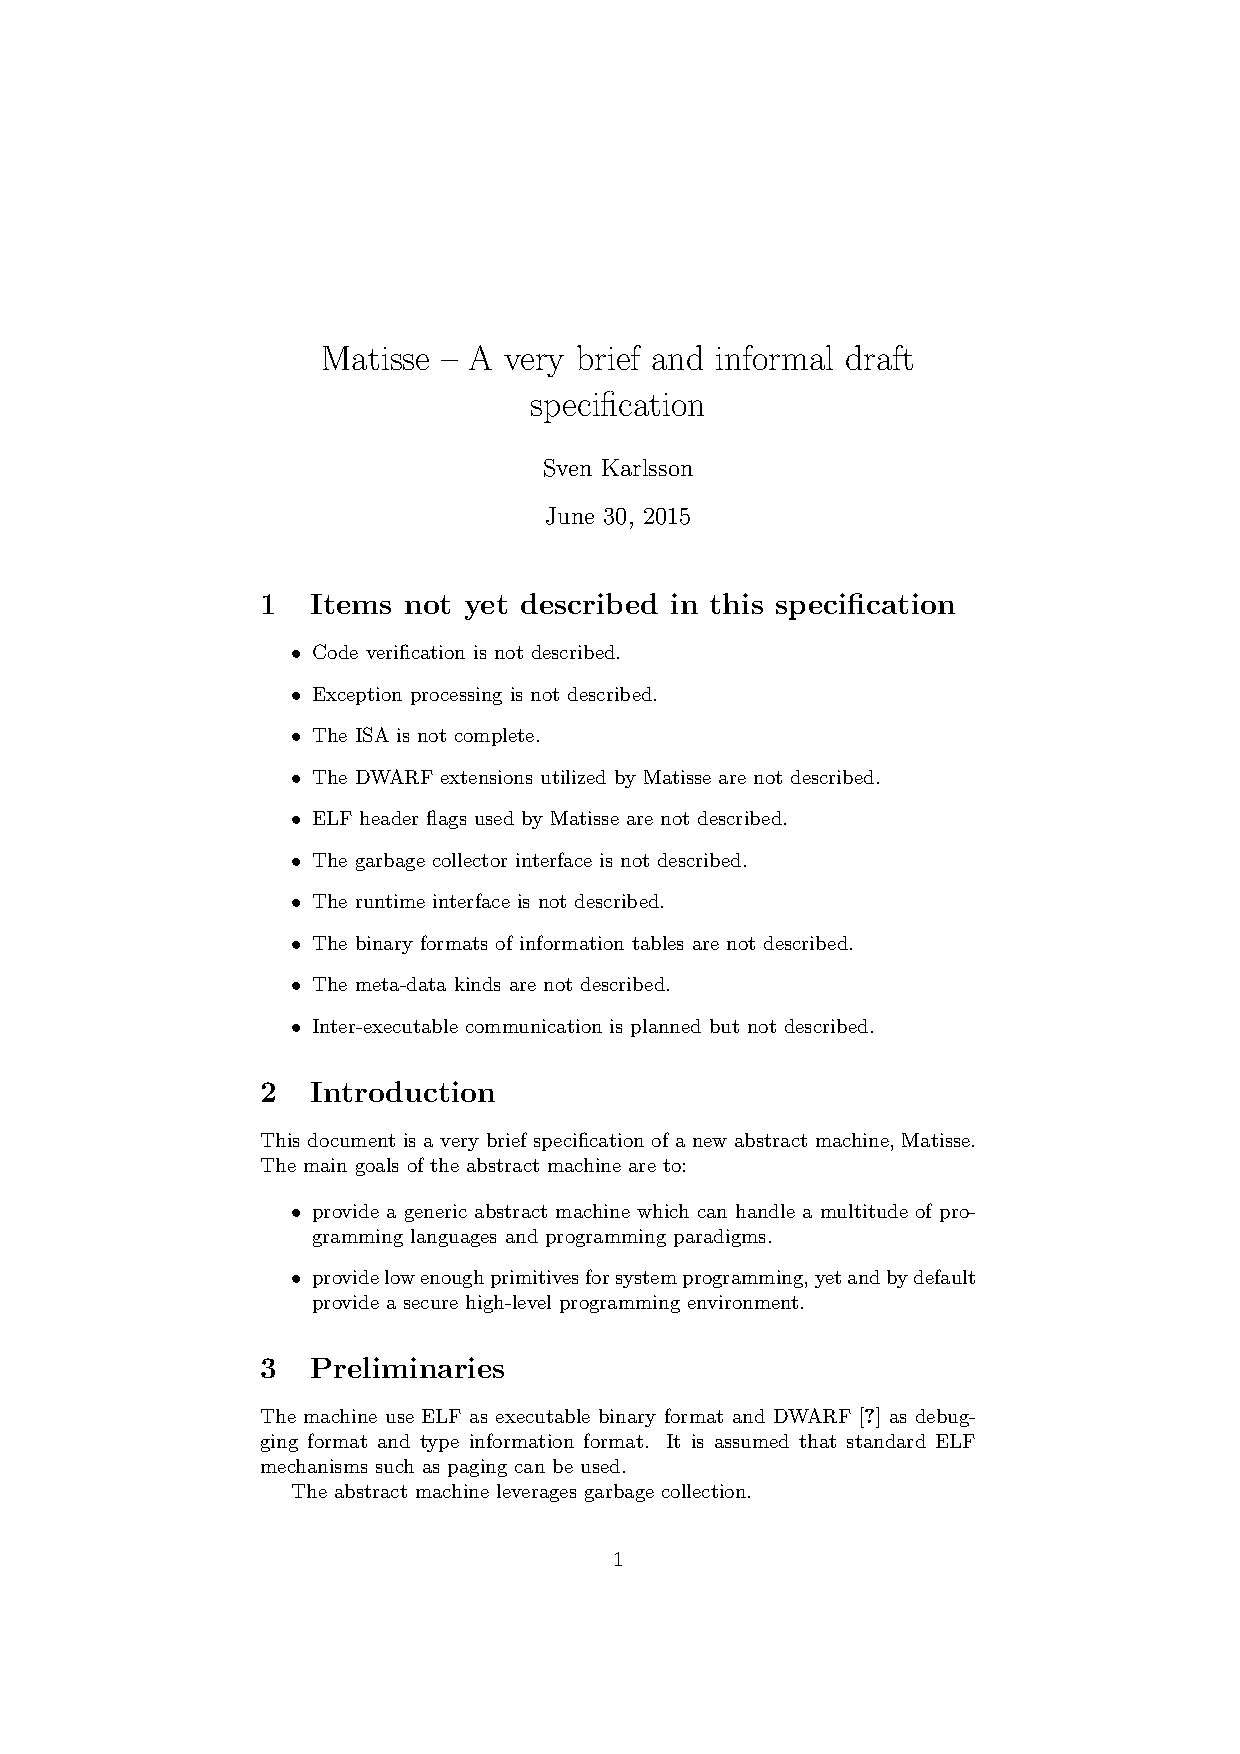
\includepdf[pages=-]{lib/spec.pdf}

\subsection{Project Inception Phase Artifact}
\label{appendix:inception-artifact}

\includepdf[pages=-]{lib/Inception.pdf}

\subsection{Benchmark Runner}
\label{appendix:benchmark}
\begin{lstlisting}[language=bash]
#!/usr/bin/bash
# benchmark runner
# based off:
# https://gist.github.com/peterjmit/3864743

repeat=1
step=1
range_from=0
range_to=30
output_file="benchmark.csv"
command=""

run_tests() {
    echo "benchmarking: ${command} ${range_from}..${range_to} (step ${step})"

    # truncate output file
    if [ -f ${output_file} ]
    then
        > ${output_file}
    fi

    # print column names
    echo "round,n,time,user,kernel" >> ${output_file}

    # repeat
    for (( j = 0; j < ${repeat}; j++ ))
    do
        # for each in range
        for (( i = ${range_from}; i < ${range_to}; i += ${step} ))
        do
            # percentage completion
            p=$(( ($i + 1) * 100 / $range_to ))
            # indicator of progress
            l=$(seq -s "#" $(($p / 2)) | sed 's/[0-9]//g')

            # time command
            /usr/local/bin/time -f "${j},${i},%e,%U,%S" -o ${output_file} -a ${command} ${i} > /dev/null

            # clear the HDD cache (i hope?)
            sync && echo 3 > /proc/sys/vm/drop_caches

            printf "%s/%s: %-48s %3s%%\r" "$(($j + 1))" "$repeat" "$l" "$p"
        done
    done

    echo -ne '\n'
}

# Option parsing
while getopts s:f:t:n:c:o: OPT
do
    case "$OPT" in
        s)
            step=$OPTARG
            ;;
        f)
            range_from=$OPTARG
            ;;
        t)
            range_to=$OPTARG
            ;;
        n)
            repeat=$OPTARG
            ;;
        o)
            output_file=$OPTARG
            ;;
        c)
            command=$OPTARG
            ;;
        \?)
            echo 'error: failed to parse args'
            exit 1
            ;;
    esac
done

shift `expr $OPTIND - 1`

if [[ $command == "" ]]
then
    echo 'error: no command to run'
    exit 1
fi

run_tests
\end{lstlisting}

%%% Local Variables:
%%% mode: latex
%%% TeX-master: "../report"
%%% End:

% Instruction set listing
% Complete backlog

\end{document}

%%% Local Variables:
%%% mode: latex
%%% TeX-master: t
%%% End:
